\documentclass[authoryearcitations]{UoYCSproject}
\usepackage[dvipdfm]{graphicx}
\usepackage[dvipdfm]{color}
\usepackage{amsmath, amsthm, amssymb}
\usepackage{a4wide}
\author{Jose Manuel Calderon}
\title{Quantum Dots as Biosensors}
\date{2011-September-14}
\supervisor{Prof. Samuel L. Braunstein}
\MNC
\wordcount{1337}
\abstract{ \LaTeXe\ is a document markup and processing system built
  upon Donald Knuth's type-setting system, \TeX.}
   


\begin{document} 
\maketitle
\chapter{Introduction}

\chapter{Literature Review}
In this chapter we will look at and discuss some of the literature relevant to this project. 
In order to properly understand the system being modeled we will briefly touch on quantum mechanics
and some of the necessary mathematics. In the second section we will look at numerical methods with
particular focus on the finite difference method\footnote{Also known as finite difference calculus.}.
We will also look at various matrix representations that are present in the tools used for our
model. 
 
\section{Quantum Dots}
Since being discovered\footnote{Some would say invented} in the 1970's by Leo Esaki and 
Raphael Tsu quantum dots have been of interest to physicists and engineers for numerous applications. 
Quantum dots (QDs from this point on) are structures of semiconductors ranging between ??????
RANGE HERE ??????. Their size and properties make them ideal in modelling atomic physics in a
macroscopic system \cite{Li}. For this reason, they are sometimes referred to as artificial atoms 
??CITE RELEVANT HERE??.

In this section we will look at the necessary concepts for modelling QDs, starting with basic 
quantum mechanics and then discuss some of the physical properties of quantum dots.

 
\subsection{Basics of Quantum Mechanics}

\subsection{Structure of Quantum Dots}


\section{Finite Difference Method}
The finite difference method is one of several numerical methods that can be used in approximating
solutions to differential equations \cite{Hamming}. We will work through the use of the finite 
difference method and then discuss why this method was chosen over other possible alternatives. 

\subsection{Background}
The finite difference method arose due to the inherent inability of computing devices to perform
calculations using infinitesimal calculus \cite{Hamming, zhilin}. Because taking the space
between two points to its limit is impossible on a computer, estimates of the derivative must be
used. Additionally, as a continuous representation of a function is not feasible, a function is represented
by sampling values of the function at discrete points. The distance between these points will
be referred to throughout this section as $h$. 


\begin{figure}[h]
  \centering
  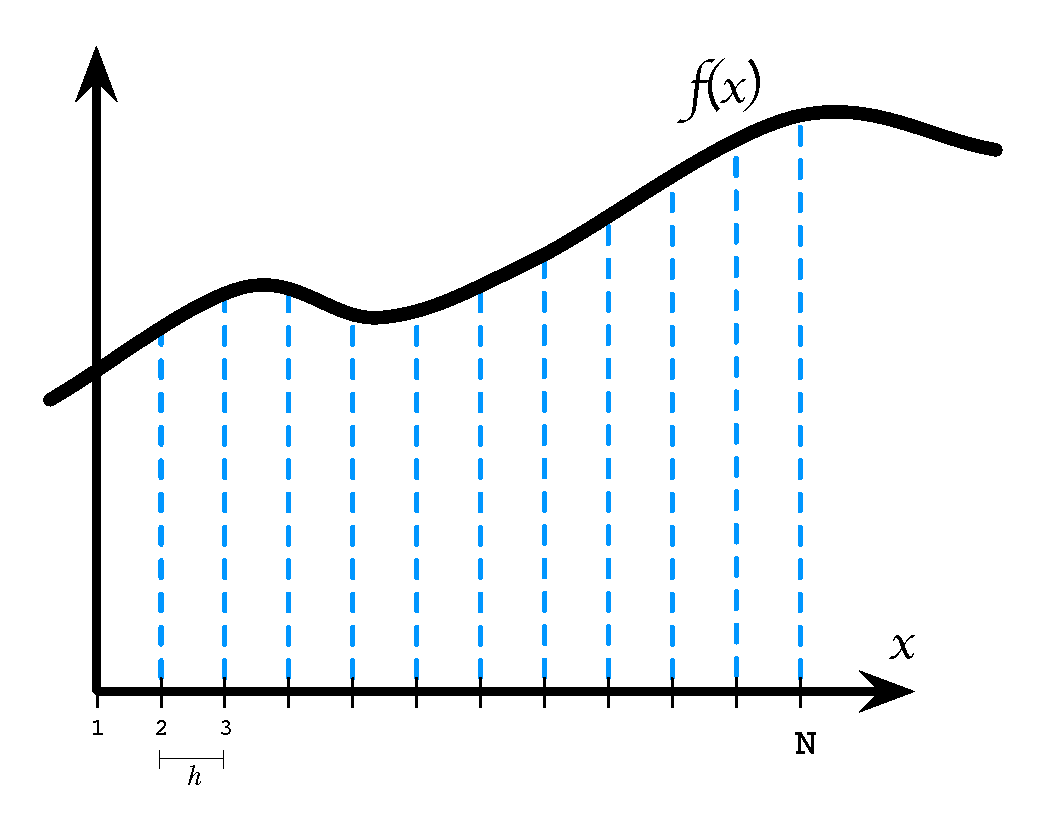
\includegraphics[scale=0.5]{figures/sampledFunc3.eps}
    \caption{Illustration of a function $f$ being sampled at discrete points}
\end{figure}

First we will define the difference operator used in FDM and then see how the difference 
operator along with the Taylor Series can be used to provide a numerical approximation of 
functions and their derivatives. 

\subsection{The Difference Operator}
A fundamental concept in the FDM is that of the difference operator. For any function 
$f$ this can be defined in three ways. As a \emph{forward difference}, a \emph{backward difference},
or as a \emph{central difference}. These are defined as follows

For the \emph{forward difference}:
\begin{equation}
\label{eq:forwardDiff}
\Delta f(x) \equiv  f(x + h) - f(x)
\end{equation}

For the \emph{backward difference}:
\begin{equation}
\label{eq:backDiff}
\nabla f(x) \equiv  f(x) - f(x - h)
\end{equation}

And for the \emph{central difference}:
\begin{equation}
\label{eq:centDiff}
\delta f(x) \equiv  f(x + \frac{1}{2}h) - f(x - \frac{1}{2}h)
\end{equation}


An important property of the difference operator that is utilized in our implementation is its linearity,
 and therefore
$$\Delta (af(x) + bg(x)) = a \Delta f(x) + b\Delta g(x) $$
where $a$ and $b$ are constants \cite{Hamming}. 

Just as with derivatives in the infinitesimal calculus, you can preform this operation repeatedly. Using the difference
operator twice, $\Delta [\Delta f(x) ] \equiv \Delta ^2 f(x) $, would correspond to the second derivative of the function. 
With the forward difference operator this is done as follows

\begin{align}
 \Delta ^2 f(x)&= \Delta [\Delta f(x)]  \nonumber\\
		&= \Delta [f(x + h) - f(x)] \nonumber\\
		&= \Delta f(x + h) - \Delta f(x) \nonumber\\  
		&= \Delta f(x + h) - (f(x + h) - f(x)) \nonumber \\
		&= f(x + 2h) - f(x + h) - (f(x + h) - f(x)) \nonumber \\ 
		&= f(x + 2h) - f(x + h) - f(x + h) + f(x) \nonumber \\
 \Delta ^2 f(x)	&= f(x + 2h) - 2f(x + h) + f(x) \label{eq:deltaSquared}
\end{align}

As we can see in equation \ref{eq:deltaSquared} the result for $\Delta ^2$ using the forward difference operator is based 
on the function's value at point $x$ and the succeeding two points $x+h$ and $x+2h$ respectively. Performing the same 
process using the central difference operator produces a slightly difference approximation

\begin{align}
 \delta ^2 f(x)&= \delta [\delta f(x)]  \nonumber\\
		&= \delta [f(x + \frac{1}{2}h) - f(x - \frac{1}{2}h)] \nonumber\\
		&= \delta f(x + \frac{1}{2}h) - \delta f(x - \frac{1}{2}h) \nonumber\\  
		&= \delta f(x + \frac{1}{2}h) - (f(x) - f(x - h)) \nonumber \\
		&= f(x + h) - f(x) - (f(x + h) - f(x)) \nonumber \\ 
		&= f(x + h) - f(x) - f(x) + f(x - h) \nonumber \\
 \delta ^2 f(x)	&= f(x + h) - 2f(x) + f(x - h)\label{eq:delta2Squared}
\end{align}


Interestingly, we can see that equations \ref{eq:deltaSquared} and \ref{eq:delta2Squared} have similar coefficients,
with each point being shifted by $-h$. Following the same steps for the backward difference would result in each point
in equation \ref{eq:deltaSquared} being shifted by $-2h$. Now that we have defined the various difference operators 
we can now apply them to approximating the derivatives of a function. 

\subsubsection{Approximating Derivatives} 
Analytically, the derivative of a function at point $x$ is the limit

\begin{equation}
  f'(x) = \lim_{h\to0} \frac{f(x + h) - f(x)}{h} \nonumber
\end{equation}

We can see that this limit looks like our forward difference operator from equation \ref{eq:forwardDiff} multiplied
by $\frac{1}{h}$. Using this form and keeping $h$ at a predetermined discrete value (not taking the limit)
is a common way of approximating the derivative \cite{Hamming, wolfram, zhilin}. Replacing the numerator with
the backward difference or the central difference provides us with approximations using those difference operators. 
Backward difference

$$f'(x) = \frac{f(x) - f(x - h)}{h} $$

Central difference

$$f'(x) = \frac{f(x + \frac{1}{2}h) - f(x - \frac{1}{2}h)}{h} $$

More generally, to approximate a function's $n^{th}$ degree derivative you must calculate the $n^{th}$ degree
difference operator and then multiply by $h^n$ \cite{Hamming, weatherley4}. For a second order derivative using
the central difference operator we are left with

\begin{equation}
f''(x) = \frac{f(x + h) - 2f(x) + f(x - h)}{h^2}
\end{equation}

The choice of which difference operator to use depends largely on the problem at hand \cite{Hamming, weatherley}. 
Some problems with specific geometric requirements may benefit from the forward or backward difference schemes \cite{weatherley}.
Weatherly uses the example of modeling advection\footnote{Advection is the transport or movement of a substance or property
(like heat or salinity) in a fluid. Convection is a subset of advection, although some use them synonymously.} as a case
where one ``must be careful to use the approximation which utilises only values that are \emph{upwind} of the point where
we wish to compute the spatial derivative'' \cite{weatherley4}. Additionally, some temporal problems may only allow
either the forward or backward difference schemes. However, in cases where a point is equally influenced
from all directions, the central difference provides more accurate solutions \cite{Hamming, weatherley, weatherley4, analysis}.
In general cases such as these, the error for the forward and backward difference schemes is $O(h)$ whereas the error 
for the central difference is $O(h^2)$ \cite{analysis, weatherley}. 
%The proofs for the error as found in \cite{weatherley} has been provided in the appendix. 

\subsection{Alternate Derivation using the Taylor Series}

Remembering the Taylor series expansion of a function

\begin{equation}
\label{eq:taylor}
f(x + h) = f(x) + f'(x)h+ \frac{f''(x)}{2!} + \frac{f'''(x)}{3!} + \dots
\end{equation}

We can `stop' the expansion at the desired derivative and solve for that derivative in order to attain an approximation. 
For example stopping at $f(x + h) = f(x) + f'(x)h$ and solving for $f'(x)$ presents us with

\begin{equation}
f'(x) = \frac{f(x + h) - f(x)}{h}
\label{eq:taylorForward}
\end{equation}



\subsection{Use with Schr\"{o}dinger Equation}

\subsection{Sources of Error}

\chapter{Implementation}

\section{Matlab}

\subsection{Linear Algebra in Matlab}


\subsection{Particle in a box}

\section{Matrix Representations}
\subsection{Sparse Matrix Representations}


\chapter{Discussion}

\chapter{Evaluation}

\chapter{Conclusion}

\bibliography{diss}

\end{document}
